%kelompok 3 kelas 3B tugas ke-2
%Diana Satima Gistivani 1154018
%M.AMRAN HAKIM SIREGAR 1154106
%INDAH RAHMAWATI 1154070
%Rizky Abdul Ghani Suherli 1154058



\section{Data Vektor}
Data vektor dalam Sistem Informasi Geografis. dalam  data vektor bumi direpresentasikan sebegai suatu  mosaic yang terdiri dari garis (arclline), polygon (dareah yang dibatasi oleh garis yang berawal dan berakhir pada titik yang sama), titik/point (node yang memiliki label),  dan nodes (titik perpotongan antara dua buah garis).Titik disimpan sebagai sepasang angka koordinat dan poligon sebagai rangkaian koordinat yang membentuk garis tertutup.Resolusi dari data vektor tergantung dari jumlah titik yang membentuk garis.
Fungsi dari vektor telah berkembang dengan pesatnya sehingga tidak hanya berfungsi sebagai sekedar outline akan tetapi telah menjadi sarana menggambarkan artistik yang sangat powerfull.Kalian juga dapat menggunakan fasilitas artistic media,yang mengolah kurva menjadi pen-style yang sangat variatif. 
\subsection{Data Raster}
Data raster merupakan data yang disimpan dalam bentuk kotak segi empat (grid)
atau sel sehingga terbentuk suatu ruang yang teratur.Pada data raster,objek geografis dipresentasikan sebagai struktur sel grid yang disebut sebagai pixel (picture element).Definisi gambar tergantung pada ukuran pixel-nya,semakin kecil ukuran permukaan bumi yang dipresentasikan oleh sel,semakin tinggi ukuran permukaannya.
\begin{figure}[ht]
\centerline{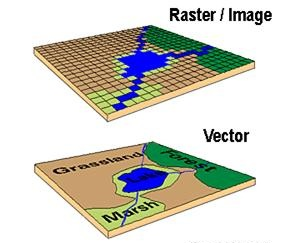
\includegraphics[width=1\textwidth] {figures/vektor01.JPG}}
\caption{tampilan dari data vektor dan data raster}
\label{vektor01}
\end{figure}
Pada gambar \ref{vektor01} ditampilkan gambar data vector dan juga data raster yang memiliki perbedaan dalam segi tampilan. Pada data raster gambar akan membentuk seperti potongan bitmap yang apabila kita melihat peta akan tidak begitu jelas di pandang, akan tetapi dalam perhitungan bisa memudahkan kita. Pada data vector gambar yang dihasilkan lebih jelas dan lebih nyata, dan dalam segi perhitungan lebih rumit karena gambar yang di hasilkan lebih jelas dan lebih nyata.
\cite{Irwansyah2013sistem}

\subsection
Model data vektor sendiri merupakan model yang banyak digunakan, model ini berbasis pada titik (points) dengan nilai koordinat (x,y) untuk membangun objek spasialnya.Objek yang dibangun terbagi menjadi tiga bagian yaitu berupa titik (point),garis (line) dan area (polygon).
\begin{enumerate}
\item Titik (point) merupakan representasi grafis yang paling sederhana pada suatu objek.Titik tidak mempunyai dimensi tetapi dapat     ditampilkan dalam bentuk simbol baik pada peta maupun dalam layar monitor.Contoh : lokasi fasilitas kesehatan.
\item Garis (Line) merupakan bentuk linear yang menghubungkan dua atau lebih titik dan merepresentasikan objek dalam satu dimensi. contoh : Jalan dan Sungai.
\item Area (Polygon) merupakan representasi objek dalam dua dimensi. contoh : Danau.
Setiap bagian dari data vektor dapat saja mempunyai informasi-informasi yang berasosiasi satu dengan lainnya seperti penggunaan sebuah label untuk menggambarkan informasi pada suatu lokasi.
\end{enumerate} 

\subsection {Perbedaan Data Vektor dan Raster}
Sistem Informasi Geografis : Prinsip Dasar dan Pengembangan Aplikasi

\subsection {Objek pada datavektor}
\begin{figure}[ht]
\centerline{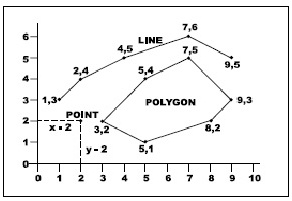
\includegraphics[width=1\textwidth] {figures/vektor02.JPG}}
\caption{tampilan skala data vektor}
\label{vektor02}
\end{figure}
Sesuai pada gambar \ref{vektor02} tergambar jelas bahwa pada penggunaan data vektor yang digunakan adalah model yang berbasis titik (point) dengan nilai koordinat (x, y).
Objek yang dibangun terbagi menjadi tiga bagian lagi, yaitu berupa titik (point), garis (line), dan area (polygon). 
\begin{enumerate}
\item titik (point) merupakan representasi grafis yang paling sederhana pada suatu objek. Titik tidak mempunyai dimensi tetapi dapat ditampilkan dalam bentuk symbol baik pada peta maupun dalam layar monitor.
\item garis (line) merupakan bentuk linear yang menghubungkan dua ataui lebih titik dan merepresentasikan objek dalam satu dimensi. 
\item Area (polygon) merupakan representasi objek dalam dua dimensi.
\end{enumerate}

\subsection { Cara Menggunaan Data Vektor}
Adapun cara menggunakan data vektor ke dalam SIG dapat dilakukan melalui tiga cara yaitu 
\begin{enumerate}
\item Penyiaman (scanning) adalah proses mengubah data grafis kontinu menjadi data grafis diskrit yang terdiri atas sel-sel penyusun gambar.
\item Digital merupakan proses pengubahan data grafis analog menjadi data grafis digital dalam struktur vektor.
\item Tabulasi adalah proses memasukkan data atribut SIG dengan pembuatan tabel.

\subsection {Aplikasi Yang Memudahkan Pembuatan Data Vektor}
\subsubsection {Microsoft Visio}
Microsoft Visio atau yang sering kita sebut visio merupakan suatu program aplikasi perangkat komputer yang memang sering digunakan atau dipakai untuk membuat sebuah diagram, misalnya seperti diagram aliran(flowchart), brainstorm, dan juga skema pada jaringan yang dikeluarkan atau dirilis oleh Microsoft Corporation. biasanya aplikasi ini memakai grafik vektor untuk menciptakan atau membuat diagram-diagramnya.
\subsubsection {Corel Draw}
CorelDraw merupakan aplikasi perangkat komputer yang juga sering digunakan sebagai pengolahan vektor. coreldraw ini juga merupakan fasilitas yang cukup sangat lengkap di bandung aplikasi yang lainnya, coreldraw juga bisa digunakan sebagai pengelolaan kurva bezier. kurva bezier (bezier curve) merupakan garing lengkung yang terbentuk dari rumusan matematis. 
kurva bezier memiliki sebuah titik pusat (anchor point) dengan garis pengendali arah atau handle. dan dari handle ini dapat kita atur seluruh kelengkungan objek melalui dua titik yang bisa di sebut sebagai titik tangen dari kurva bezier ini.

\subsection{Kekurangan dan Kelebihan Data Vektor}
\subsubsection{Kelebihan Data Vektor}
Kelebihan data vektor di bandingkan data raster
data vektor relatif lebih ekonomis dalam hal ukuran file dan presisi dalam lokasi, tetapi sangat sulit untuk digunakan dalam komputasi matematik. 
\begin{enumerate}
\item Mempunyai struktur data yang sangat sederhana.
\item sangat mudah dimanipulasi dengan menggunakan fungsi-fungsi matematis yang sederhana.
\item pada data vector teknologi yang digunakan sangat  murah dan tidak begitu kompleks sehingga pengguna.
\item bisa membuat sendiri program aplikasi yang mengunakan citra raster.
\item cocok atau sesuai dengan citra-citra satelit penginderaan jauh dan semua image hasil scanning data spasial.
\item  memiliki kombinasi data raster dengan data inderaja mudah dilakukan
\item mempunyai beberapa kemampuan-kemampuan permodelan dan analisis spasial tingkat lanjut.
\item pada data vektor metode untuk mendapatkan citra raster lebih mudah.
\item model permukaan bumi di dalam bentuk citra raster yang didapat dari radar atau satelit penginderaan jauh selalu lebih actual dari pada bentuk vektornya
\item Prosedur untuk memperoleh data dalam bentuk raster lebih mudah, sederhana dan murah.
\item Harga system perangkat lunak aplikasinya cenderung lebih murah.
\item Memiliki resolusi spasial yang tinggi.
\item Transformasi koordinat dan proyeksi tidak sulit dilakukan.
\item Hubungan topologi dan network dapat dilakukan dengan mudah.
\end{enumerate}
\subsubsection{Kekurangan data Vektor}
kekurangan data vector dibandingkan data raster
terdapat keterbatasan masalah akurasi dan presisi data terutama dalam menentukan ukuran piksel. Data vector memiliki keterbatasan dalam ukuran penyimpanan atau kapasitas hasil.
\begin{enumerate}
\item Memiliki struktur data yang kompleks.
\item Datanya tidak mudah untuk dimanipulasi.
\item Pengguna tidak mudah berkreasi untuk membuat programnya sendiri untuk memenuhi kebutuhan aplikasinya. Hali ini disebabkan oleh struktur data vector yang lebih kompleks dan prosedur fungsi dan analisisnya memerlukan kemampuan tinggi karena lebih sulit. Pengguna harus membeli system perangkat lunaknya karena teknologinya masih mahal.
\item Prosedurnya pun terkadang lebih sulit. Karena proses keseluruhan untuk mendapatkannya lebih lama, peta vector seringkali mengalami out of date atau kadaluarsa.
\item Memerlukan perangkat keras dan perangkat lunak yang lebih mahal.
\item Overlay beberapa layers vector secara simultan memerlukan waktu yang relative lama.
\item Karena proses keseluruhan untuk mendapatkannya lebih lama,peta vektor seringkali mengalami out of date atau kadaluarsa.
\item data ini adalah ketidakmampuannya dalam mengakomodasi perubahan fenomena yang bersifat gradual.
\end{enumerate}

\subsection{Model Data Vektor}
\begin{figure}[ht]
\centerline{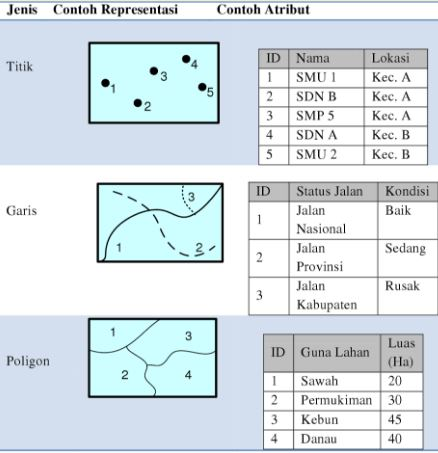
\includegraphics[width=1\textwidth] {figures/vektor03.JPG}}
\caption{representasi data vektor dan atributnya}
\label{vektor03}
\end{figure}
Sesuai dengan gambar \ref{vektor03} model data vector terbagi menjadi beberapa bagian
\begin{enumerate} 
\item Topologi, biasa digunakan dalam analisis spasial dalam SIG. topologi adalah model data vector yang menunjukan hubungan spasial di antara objek spasial. Topologi sangat berguna pada saat melakukan seteksi kesalahan ketika proses digitasi, dan berguna pula dalam melakukan proses analisis spsial.
Model data vektor dalam topologi dikembangkan dalam dua kategori,yaitu Data Sederhana (Simple Data) yang merupakan representasi data yang mengandung tiga jenis data (titik,garis,poligon) secara sederhana.Sedangkan Data Tingkat Tinggi (Higher Data Level),dikembangkan lebih jauh dalam melakukan pemodelan secara tiga dimensi (3 Dimensi/3D).
\item Non Topologi, adalah model data yang mempunyai sifat yang lebih cepat dalam menampilkan dn dpat digunakan secara langsung dalam perangkat lunak (software) SIG yang berbeda-beda.
\item Region, adalah sekumpulan polygon, dimana masing-masing polygon dapat atau tidak mempunyai kaitan di antaranya akan tetapi saling bertampalan dalam satu data set.
\item Dynamis Segmentation, merupakan model data yang dibangun dengan menggunakan garis dalam rangka membangun model jaringan (network).
\item Model data vektor dekenal pula dengan model data spagetti.Pada model ini,lembaran kertas peta ditranslasikan garis-garis 
ke dalam list koordinat (x,y) dalam format digital.Sebuah titik dikodekan sebagai pasangan koordinat (x,y) tunggal.Sementara area atau ulasan dikodekan sebagai poligon dan direkam sebagai pasangan koordinat closed-loop yang didefinisikan batas-batasannya.
\end{enumerate}
\cite{Janner2010rekayasa}

\subsection
klasifikasi model data spasial dibagi menjadi dua bagian yaitu data vektor dan model data raster, kemudian data vektor dibagi menjadi dua bagian, yaitu non-topologi dan topologi. Kemudian data topologi tersebut dibagi lagi menjadi dua bagian yaitu data sederhana(simple data) dan data tingkat tinggi(higher data level), lalu data tingkat tinggi di bagi menjadi tiga bagian, yaitu TIN(tringulated irregular network), regions, dan dynamic segmentation. Itulah klasifikasi model data spasial yang di dalamnya banyak sekali bagian yang sangat spesifik, sehingga klasifikasi model data spasial ini bisa di katagorikan sebagai klasifikasi model yang sangat kompleks.

\subsection 
pada data vektor ini, kita dapat simpulkan bahwa penggunaan suatu aplikasi dapat di sesuaikan dengan apa saja hal-hal yang kita perlukan dan kita inginkan agar dapat sesuai pada proses dan juga hasilnya yang kita harapkan. Sehingga data data yang telah di kumpulkan dapat digunakan untuk keperluan sistem informasi geografis yang sangat lengkap.

\subsection
pada data vektor yang dijelaskan bahwa data berikut merupakan data yang valid dengan menggunakan model data spasial dengan menggunakan titik, dan meyimpan dat asapsial menggunakan garis-garis atau kurva atau pologion beserta atribut-atributnya. bentuk- bentuk dasar sepsertasi data yang ada data spasial ini, didalam sistem dalam ini dalam ssistem kordinat data vektor. jarak antara rumah didesa sistem perhubungannya dan kondisi geografis.
\cite{Budiyanto2002sistem}
